\clearpage
\maketitlesupplementary

\renewcommand\thesection{\Alph{section}}
\renewcommand\thetable{\Alph{table}}
\renewcommand\thefigure{\Alph{figure}}
\renewcommand\theequation{\Alph{equation}}
\setcounter{section}{0}
\setcounter{table}{0}
\setcounter{figure}{0}
\setcounter{equation}{0}


% --- ADD THIS LINE TO CREATE THE APPENDIX TOC ---
\tableofcontents
% -----------------------------------------------

% Helper for boxed imagery in the supplementary
\begingroup
\makeatletter
\setlength{\@fptop}{0pt}
\makeatother
\setlength{\fboxrule}{0.4pt}
\let\oldincludegraphics\includegraphics
\renewcommand{\includegraphics}[2][]{%
  \setlength{\fboxsep}{0pt}%
  \fbox{\oldincludegraphics[#1]{#2}}}

\newpage  

\section{Video Demo}
\label{app:demo-screenshots}

We have created a web-app based on PPTPilot (Sec.~\ref{sec:pptpilot}), which can convert a given PPT according to the user instructions. Please refer to the \textbf{videos in our supplementary materials} for their process. In our Fig.~\ref{fig:pptpilot_demo_screenshots}, we have illustrated the webapp conducting chat-based editing for users' provided PPTs and how PPTArena runs the evaluation by comparing the ground truth and prediction slides.
  
  % Changed [t] to [!ht] to force it BELOW the section title
  \begin{figure}[!ht]
      \centering
      \begin{minipage}{0.95\linewidth}
          \centering
          \includegraphics[width=\linewidth]{figures/PPTPilotChatDemo.jpg}
          \vspace{0.35em}
          {\small Chat-based Editing}
      \end{minipage}
      \hfill
      \begin{minipage}{0.95\linewidth}
          \centering
          \includegraphics[width=\linewidth]{figures/PPTPilotWebpage.jpg}
          \vspace{0.35em}
          {\small PPTArena Evaluation}
      \end{minipage}
      \caption{Our WebApp Demo for PPTPilot in chat-based editing (Top) and PPTArena evaluation (bottom). See the \protect\hyperlink{pptarena-code}{PPTArena codebase}
and the \protect\hyperlink{pptarena-web}{project webpage}.}
      \label{fig:pptpilot_demo_screenshots}
  \end{figure}


\begin{table*}[!htbp]
\centering
\small
\setlength{\tabcolsep}{6pt}
\renewcommand{\arraystretch}{1.2}
\caption{{\bf Detailed VLM-as-Judge Evaluation Results (Gemini 2.5 Pro)}. Scores report instruction-following (IF) and visual quality (VQ) with VLM-as-judge. Columns marked with $^{*}$ are only run on a 25-case subsample for cost and rate-limit reasons. Bracketed values in the PPTPilot column report scores on that same subsample.}
\vspace{-2mm}
\label{tab:gemini2.5proasEvals}
\resizebox{\linewidth}{!}{%
\begin{tabular}{l r
    >{\columncolor{cyan!9}}c >{\columncolor{cyan!9}}c  % PPTPilot
    >{\columncolor{gray!12}}c   >{\columncolor{gray!12}}c    % Gemini
    >{\columncolor{orange!12}}c   >{\columncolor{orange!12}}c    % ChatGPT
    >{\columncolor{green!8}}c   >{\columncolor{green!8}}c    % ChatGPT Agent
    >{\columncolor{purple!10}}c >{\columncolor{purple!10}}c  % Mini Max Agent
    c c  % PPTAgent*
    c c  % Poster2Agent*
}
\toprule
& & \multicolumn{2}{c}{\textbf{PPTPilot}}
  & \multicolumn{2}{c}{\textbf{Gemini CLI}}
  & \multicolumn{2}{c}{\textbf{ChatGPT}}
  & \multicolumn{2}{c}{\textbf{ChatGPT Agent$^{*}$}}
  & \multicolumn{2}{c}{\textbf{MiniMax Agent$^{*}$}}
  & \multicolumn{2}{c}{\textbf{PPTAgent$^{*}$}}
  & \multicolumn{2}{c}{\textbf{Poster2Agent$^{*}$}} \\
\cmidrule(lr){3-4}\cmidrule(lr){5-6}\cmidrule(lr){7-8}\cmidrule(lr){9-10}\cmidrule(lr){11-12}\cmidrule(lr){13-14}\cmidrule(lr){15-16}
\textbf{Category} & \textbf{Cases} & IF$\uparrow$ & VQ$\uparrow$ & IF$\uparrow$ & VQ$\uparrow$ & IF$\uparrow$ & VQ$\uparrow$ & IF$\uparrow$ & VQ$\uparrow$ & IF$\uparrow$ & VQ$\uparrow$ & IF$\uparrow$ & VQ$\uparrow$ & IF$\uparrow$ & VQ$\uparrow$ \\
\midrule
Content      & 67 &
\textbf{2.51}\hspace{0.15em}[\textbf{2.10}] & \textbf{2.68}\hspace{0.15em}[\textbf{2.35}] &
1.93 & 2.14 &
1.95 & 2.00 &
1.45 & 1.65 &
0.90 & 0.80 &
0.00 & 0.00 &
0.00 & 0.00 \\
Layout       & 29 &
\textbf{2.18}\hspace{0.15em}[\textbf{2.00}] & \textbf{2.64}\hspace{0.15em}[\textbf{2.14}] &
1.89 & 2.07 &
1.96 & 2.00 &
0.86 & 0.86 &
0.86 & 0.57 &
0.00 & 0.00 &
0.00 & 0.00 \\
Styling      & 29 &
\textbf{2.54}\hspace{0.15em}[\textbf{2.17}] & \textbf{2.50}\hspace{0.15em}[\textbf{2.33}] &
2.17 & 2.07 &
2.37 & 1.85 &
0.83 & 0.83 &
1.00 & 0.83 &
0.00 & 0.00 &
0.00 & 0.00 \\
Structure    & 15 &
\textbf{2.47}\hspace{0.15em}[1.67] & \textbf{3.60}\hspace{0.15em}[\textbf{2.33}] &
1.87 & 2.33 &
1.80 & 1.53 &
\textbf{2.00} & 1.67 &
0.67 & 0.67 &
0.00 & 0.00 &
0.00 & 0.00 \\
Interactivity& 4 &
2.00\hspace{0.15em}[\textbf{2.00}] & 3.00\hspace{0.15em}[\textbf{2.00}] &
1.00 & 2.25 &
\textbf{2.25} & \textbf{4.25} &
1.00 & \textbf{2.00} &
0.00 & 0.00 &
0.00 & 0.00 &
0.00 & 0.00 \\
\midrule
All Cases    & 100 &
\textbf{2.45}\hspace{0.15em}[\textbf{2.04}] & \textbf{2.74}\hspace{0.15em}[\textbf{2.60}] &
1.92 & 2.15 &
1.97 & 2.03 &
1.44 & 1.32 &
0.92 & 0.80 &
0.00 & 0.00 &
0.00 & 0.00 \\
\bottomrule
\end{tabular}}
\vspace{-2mm}
\end{table*}

\section{PPTPilot Analysis}

\subsection{Gemini 2.5 Pro as Judge}

In our main paper, we utilize GPT as the VLM judge (Table~\ref{tab:pptpilot_ablation}) for PPTArena. To validate the robustness of our PPTPilot, we conduct a further experiment using Gemini 2.5 Pro as the VLM judge. As shown in Table~\ref{tab:gemini2.5proasEvals}, we conduct the same set of experiments as in Table~\ref{tab:pptpilot_ablation} and highlight the following observations. As clearly shown, PPTPilot still shows a significant advantage over other approaches, including the proprietary agents. This suggests that our PPTPilot is simple yet effective. \Cref{fig:gemini_barplots} visualizes the alignment between scores assigned by different VLM judges. The comparison demonstrates that while absolute score values may vary slightly between judges, the relative ranking of agents remains consistent, with PPTPilot maintaining its lead across both the full benchmark and the challenging subset.

\subsection{PPTPilot on T2US}

In Table~\ref{tab:pppilot-vs-t2us}, we compare PPTPilot on the T2US~\cite{jung2025talkslideslanguagedrivenagents} benchmark. We adopt \textit{gemini-2.5-flash} as our backbone model, the same as T2US, for a fair comparison. As clearly demonstrated, our PPTPilot has a significant advantage over T2US, achieving better quality, exceeding a score of 4 out of 5 in multiple categories. In fact, this also demonstrates the need for our PPTArena to introduce more challenging PPT editing scenarios. 

\begin{table}[t]
\centering
\caption{\textbf{PPTPilot vs.\ T2US on the T2US benchmark.}
We report success rate and judge ratings for different quality dimensions.}
\vspace{-2mm}
\label{tab:pppilot-vs-t2us}
\resizebox{\columnwidth}{!}{%
\begin{tabular}{lcc}
\toprule
\multirow{2}{*}{Metric} & \multicolumn{2}{c}{T2US Benchmark} \\
\cmidrule(lr){2-3}
 & T2US~\cite{jung2025talkslideslanguagedrivenagents} & PPTPilot (ours) \\
\midrule
Success rate (\%)              & 96.83          & \textbf{100.00} \\
Instruction following $\uparrow$ & 2.21           & \textbf{4.05}   \\
Image quality $\uparrow$         & 2.17           & \textbf{4.44}   \\
Layout quality $\uparrow$        & 2.58           & \textbf{4.40}   \\
Color quality $\uparrow$         & 2.57           & \textbf{4.20}   \\
Text quality $\uparrow$          & 2.48           & \textbf{3.92}   \\
\bottomrule
\end{tabular}%
}
\vspace{-3mm}
\end{table}


\section{PPTArena Analysis}

\subsection{Challenging Scenario Distribution}
We analyze how the difficulty levels of editing categories are distributed in our benchmark. Table~\ref{tab:difficulty_by_category} shows that Structure and Interactivity require the longest programs (6.8--7.2 operations on average) and span the most slides (10--11), which leads to the highest cross-slide and high-diff rates (56--70\% and 71--75\%). Content, Layout, and Styling remain challenging, with roughly one-third of cases requiring cross-slide consistency (26--34\%) and 41--52\% tagged as high-diff. Overall, PPTArena focuses on multi-slide and multimodal reasoning tasks rather than inflating the benchmark with easier single-slide tweaks. 


\subsection{Comparison with Related Benchmarks}

In Table~\ref{tab:benchmark_landscape}, we compare our PPTArena with existing PPT-related benchmarks and highlight its uniqueness, providing further details in Table~\ref{tab:edit_difficulty_comparison}. As clearly demonstrated, our PPTArena provides broader coverage of scenarios, does not rely on predefined APIs or COMs, and is based on a larger number of source slides. In addition, our evaluation protocol is carefully designed to enable rigorous, reliable evaluation by providing detailed ground truth, predictions, and per-sample style-targets for reproducible scoring.

Notably, prior benchmarks, \emph{e.g.}, PPTC-R, might not be challenging enough given the progress of VLMs. Specifically, we evaluate GPT-5 and Gemini 2.5 Pro using PPTC-R's pipeline and achieved the success rates of 92\% and 88\%, respectively. These observations further suggest the necessity of building a challenging PPT editing benchmark like our PPTArena.




\begin{table}[t]
\centering
\small
\setlength{\tabcolsep}{4pt}
\renewcommand{\arraystretch}{1.1}
\caption{\textbf{Challenge distribution in PPTArena.} For each editing category, we report the average number of operations and slides touched per case, along with the share of cases tagged as cross-slide or high-diff. Cross-slide cases require coordinated semantic edits across at least two slides (for example, including visuals based on prior slides or consolidating charts). High-diff is a deterministic flag for cases that combine long-horizon programs or strong text-visual dependencies, as in Table~\ref{tab:edit_difficulty_comparison}.}
\label{tab:difficulty_by_category}
\resizebox{0.9\linewidth}{!}{%
\begin{tabular}{l r c c c c}
\toprule
\textbf{Category} & 
\multicolumn{1}{c}{\rotatebox{90}{\textbf{Cases}}} & 
\multicolumn{1}{c}{\rotatebox{90}{\textbf{Avg. ops}}} & 
\multicolumn{1}{c}{\rotatebox{90}{\textbf{Avg. slides}}} & 
\multicolumn{1}{c}{\rotatebox{90}{\textbf{Cross-slide}}} & 
\multicolumn{1}{c}{\rotatebox{90}{\textbf{High-diff.}}} \\
\midrule
Content        & 67 & 4.3 & 6.8 & 26\% & 41\% \\
Layout         & 29 & 5.7 & 8.9 & 34\% & 52\% \\
Styling        & 29 & 5.1 & 9.4 & 30\% & 48\% \\
Structure      & 15 & 6.8 & 11.2 & 56\% & 71\% \\
Interactivity  & 4  & 7.2 & 10.5 & 70\% & 75\% \\
\midrule
All tags (multi-label) & 144 & 5.1 & 8.3 & 32\% & 49\% \\
\bottomrule
\end{tabular}%
}
\vspace{-4mm}
\end{table}




\begin{table*}[t]
    \centering
    \small
    \setlength{\tabcolsep}{6pt}
    \renewcommand{\arraystretch}{1.1}
    \caption{\textbf{Benchmark and evaluation coverage comparison.}
    We contrast PPTArena with prior PowerPoint editing / generation benchmarks in terms of scenario focus and what aspects of evaluation they make observable vs.\ leave under-specified.}
    \vspace{-3mm}
    \label{tab:benchmark_landscape}
    \resizebox{\linewidth}{!}{%
    \begin{tabular}{l p{0.30\linewidth} p{0.47\linewidth}}
    \toprule
    \textbf{Benchmark} & \textbf{Scenario focus} & \textbf{Evaluation coverage and gaps} \\
    \midrule
    PPTC-R~\cite{zhang-etal-2024-pptc}
    & Macro playback of $<\!100$ API functions on templated decks
    & Regenerates decks via Office macros and checks API diffs, but does not release PPTX pairs or manifests. Outputs can vary by Office build, and there is no direct semantic or visual quality judgment. \\
    \addlinespace[2pt]
    TSBench (Talk to Your Slides)~\cite{jung2025talkslideslanguagedrivenagents}
    & COM-scripted instruction following on 379 prompts over corporate templates
    & Lacks dual scoring and public reference slides; edits rarely exceed four operations per case, and 379 prompts are extrapolated from 56 underlying edit tasks, limiting diversity and compositional difficulty. \\
    \addlinespace[2pt]
    Paper2Poster~\cite{pang2025paper2postermultimodalposterautomation}
    & Single-slide poster generation from research papers
    & Uses a QA pipeline plus a single VLM-as-judge. Scoring is coarse, with no structured manifests or per-operation fidelity, and the benchmark is not designed for multi-step editing or layout-preserving updates. \\
    \addlinespace[2pt]
    AutoPresent~\cite{ge2025autopresentdesigningstructuredvisuals}
    & SlidesBench: prompts derived from existing slides for PPT generation from scratch
    & Reports spatial/text/color metrics and heuristic checks, but reference decks and judge rationales are not publicly released (subscription only), and the reported test set contains just 10 PowerPoint decks. \\
    \addlinespace[2pt]
    PPTAgent~\cite{pptagent2025}
    & Document-to-slide synthesis via a hierarchical presentation agent
    & PPTEval uses a single LLM to rate content/design/coherence, without deterministic manifests, accessibility checks, or explicit visibility into which elements were inserted, modified, or preserved. \\
    \midrule
    \textbf{PPTArena (ours)}
    & 100-case, 2{,}125-slide multi-edit benchmark covering 16 edit types across 5 categories
    & Releases Original / Prediction / Ground-truth PPTX triplets, style-target manifests, and dual VLM judges: IF (instruction-following via structured JSON/XML diffs) and VQ (visual quality via screenshots). Supports reproducible, traceable scoring, hybrid API/XML evaluations, and iterative verification under realistic multi-edit workloads. \\
    \bottomrule
    \end{tabular}}
\end{table*}


\begin{figure*}[!htbp]
    \centering
    \begin{minipage}{0.98\linewidth}
    \setlength{\fboxsep}{0pt}
    \vspace{0.4em}
    \rule{0.98\linewidth}{0.5pt}

    \vspace{0.4em}

    \begin{tabular}{@{}p{0.48\linewidth}p{0.48\linewidth}@{}}

    % ===================== ROW 1 =====================
    % Object Distance (left)
    \begin{minipage}[t]{\linewidth}
        \textbf{\normalsize Object Distance (16 slides total)}\\
        \begin{minipage}[t]{0.48\linewidth}
            \centering
            {\small Original}\\[0.3em]
            \includegraphics[page=1,width=\linewidth]{figures/ObjectDistance_TestA.pdf}\\[0.2em]
            \includegraphics[page=14,width=\linewidth]{figures/ObjectDistance_TestA.pdf}
        \end{minipage}%
        \hfill
        \begin{minipage}[t]{0.48\linewidth}
            \centering
            {\small Ground Truth}\\[0.3em]
            \includegraphics[page=1,width=\linewidth]{figures/ObjectDistance_GTA.pdf}\\[0.2em]
            \includegraphics[page=14,width=\linewidth]{figures/ObjectDistance_GTA.pdf}
        \end{minipage}
    \end{minipage}
    &
    % Update Theme (right)
    \begin{minipage}[t]{\linewidth}
        \textbf{\normalsize Update Theme (28 slides total)}\\
        \begin{minipage}[t]{0.48\linewidth}
            \centering
            {\small Original}\\[0.3em]
            \includegraphics[page=22,width=\linewidth]{figures/updatetheme_TestA.pdf}\\[0.2em]
            \includegraphics[page=27,width=\linewidth]{figures/updatetheme_TestA.pdf}
        \end{minipage}%
        \hfill
        \begin{minipage}[t]{0.48\linewidth}
            \centering
            {\small Ground Truth}\\[0.3em]
            \includegraphics[page=22,width=\linewidth]{figures/updatetheme_GroundTruthA.pdf}\\[0.2em]
            \includegraphics[page=27,width=\linewidth]{figures/updatetheme_GroundTruthA.pdf}
        \end{minipage}
    \end{minipage}
    \\[1.2em]

    % ===================== ROW 2 =====================
    % Dynamic Chart Conversions (left)
    \begin{minipage}[t]{\linewidth}
    \vspace{0.2em}
        \textbf{\normalsize Dynamic Chart Conversions (5 slides total)}\\
        \begin{minipage}[t]{0.48\linewidth}
            \centering
            {\small Original}\\[0.3em]
            \includegraphics[page=1,width=\linewidth,trim=0cm 1.8cm 0cm 0cm,clip]{figures/ChangeLineGraphtoBar_TestA.pdf}\\[0.2em]
            \includegraphics[page=3,width=\linewidth,trim=0cm 1.5cm 0cm 1cm,clip]{figures/PieChart_TestA.pdf}
        \end{minipage}%
        \hfill
        \begin{minipage}[t]{0.48\linewidth}
            \centering
            {\small Ground Truth}\\[0.3em]
            \includegraphics[page=1,width=\linewidth,trim=0cm 1.8cm 0cm 0cm,clip]{figures/ChangeLineGraphtoBar_GroundTruthA.pdf}\\[0.2em]
            \includegraphics[page=3,width=\linewidth,trim=0cm 1.5cm 0cm 1cm,clip]{figures/PieChart_GroundTruthA.pdf}
        \end{minipage}
    \end{minipage}
    &
    % Translate Arabic LTR (right)
    \begin{minipage}[t]{\linewidth}
    \vspace{0.2em}
        \textbf{\normalsize Translate Arabic LTR (22 slides Total)}\\
        \begin{minipage}[t]{0.48\linewidth}
            \centering
            {\small Original}\\[0.3em]
            \includegraphics[page=5,width=\linewidth]{figures/TranslateArabicLTR_TestB.pdf}\\[0.2em]
            \includegraphics[page=17,width=\linewidth]{figures/TranslateArabicLTR_TestB.pdf}
        \end{minipage}%
        \hfill
        \begin{minipage}[t]{0.48\linewidth}
            \centering
            {\small Ground Truth}\\[0.3em]
            \includegraphics[page=5,width=\linewidth]{figures/TranslateArabicLTR_GroundTruthB.pdf}\\[0.2em]
            \includegraphics[page=17,width=\linewidth]{figures/TranslateArabicLTR_GroundTruthB.pdf}
        \end{minipage}
    \end{minipage}
    \end{tabular}

    \vspace{0.6em}
    \rule{0.98\linewidth}{0.5pt}
    \end{minipage}

    \caption{Example edit queries in PPTArena, including correcting object distances, changing plot styles, updating PPT themes, and translating the contents. As demonstrated, our PPTArena contains a wide range of slide decks with varied visual elements and content. PPT editing operations are also typically spread across multiple pages, underscoring the challenge of reliable PPT editing in the real world.}
    \label{fig:pptarencases}
\end{figure*}










%%%%%%%%%%%%%%%%%%%%%%%%%%%%%%%%%%%%%%%%%%%%%%%%%%%%%%%%%%%%
\section{PPTArena Dataset Construction}
\label{app:dataset}

We detail the multi-stage construction of PPTArena (supplementing Sec.~\ref{sec:benchmark}), covering data sourcing, curation, and the extraction pipeline to derive rubrics for evaluation illustrated in \Cref{lst:pptx_to_json}.

\subsection{Data Sources and Licensing}

\begin{itemize}
    \item \textbf{Zenodo}: We sourced open-access presentations from Zenodo repositories.
    \item \textbf{Government and Educational Sources}: We collected PPTs from .gov and .edu domains to ensure a variety of formal and academic styles.
    \item \textbf{Web Scraping}: We utilized targeted search queries to find relevant financial and business presentations, such as:
    \begin{quote}
        \texttt{'quarter revenues' filetype:pptx}
    \end{quote}
    \item \textbf{Creative Licenses}: We included high-quality templates and decks from Slideshare and SlidesCarnival that are available under Creative Commons Licenses.
    \item \textbf{Student Contributions}: We curated presentations from students in diverse fields like Biology, Art Practice, and Chemical Engineering to capture different disciplinary norms.
\end{itemize}

\subsection{PPT and Scenario Curation}

\mypar{PPT Selection.} In our initial sourcing, we have gathered a database with more than 15k PPTs. To select the proper ones for building a high-quality evaluation benchmark, we first convert the PPT files to a structured JSON format and retain only those with multimodal elements, such as images, tables, charts, and customized themes. Then we ranked the PPTs according to their file size, number of slides, and content variety, leading to the top 500 most diverse slide decks. Finally, a team of human annotators manually inspected the candidate decks based on the following criteria and picked the top 100 PPTs for editing: (1) \emph{Quality}: Rejecting decks with broken layouts, low-resolution images, and unreadable texts; (2) \emph{Privacy}: Removing any decks containing personal information; (3) \emph{Complexity}: Prioritizing slides that offer interesting elements (\emph{e.g.}, complex charts, grouped shapes). After this process, we curate a set of high-quality PPTs ready for evaluating the editing challenge.

\mypar{Editing Query Creation.} By providing the respective categories and edit types listed in table~\ref{tab:edit_taxonomy}, we use a combination of AI-generated prompts and human-inspired edits to come up with all of our queries. For each category, we use multiple AI models, prompting each for high-fidelity, multi-step, hard-reasoning tasks. We manually validated more than 200 of these prompts. Then through a selection process of combining and fitting prompts to PPTs we reduced this to our curated 100 case set.

% \subsection{Distribution and Difficult Labeling}

% \mypar{Taxonomy of Edits}: We design the taxonomy of edits (Table~\ref{tab:edit_taxonomy}) real-world editing workflows to define a taxonomy of 16 distinct edit types, grouped into 5 high-level categories:
%     \begin{enumerate}
%         \item \textbf{Content}: Text editing, summarization, translation, data updates.
%         \item \textbf{Layout}: Alignment, resizing, reordering, grid application.
%         \item \textbf{Styling}: Color changes, font updates, theme application.
%         \item \textbf{Structure}: Adding/deleting slides, merging presentations.
%         \item \textbf{Interactivity}: Animations, transitions, hyperlinks.
%     \end{enumerate}
\mypar{Distribution.} We ensured that each category (Table~\ref{tab:edit_taxonomy}) is well-represented, with at least 2 cases for every specific edit type. The benchmark is weighted towards the most common and challenging edit types in the real world. As shown in Fig.~\ref{fig:pptarencases}, our PPTArena covers a wide range of requests and shows a wide variety of visual elements for editing. 

\mypar{Difficulty Labeling.} For each case we record four aligned signals: (1) the number of atomic operations in the ground-truth program, (2) the number of distinct slides edited, (3) whether the instruction or style target imposes cross-slide dependencies (updates on one slide conditioned on content in another or deck-wide consistency requirements), and (4) a \emph{high-diff} (high difficulty) flag. We designate a case as high-diff when a task contains cross-slide dependencies or heavy visual-textual semantic reasoning dependencies, such as chart remapping or translation. These consistent labels produce the distribution summarized in Table~\ref{tab:difficulty_by_category}.


\subsection{Ground-Truth Deck Creation}
Our benchmark consists of 100 cases. 80 are derived from real-world slide decks (domain-specific presentations or web-sourced), and 20 are synthetically generated using \texttt{python-pptx} to provide a controlled baseline. For the real-world decks, expert human annotators manually performed edits to create the Ground Truth, each of which typically took more than 2 hours. This ensures that the target state reflects high-quality, human-level design decisions. For the 20 synthetic cases, the ground-truth PPTs were generated by programs, providing a reliable reference.

\subsection{Subset Evaluation Data Setup}
By default, we utilize all of the PPTs in our benchmark for a full evaluation of agents. However, we curate a subset catering to the strict rate limits and cost of proprietary agents. Specifically, we define a ``hard'' subset of 25 cases that represents the most difficult scenarios in PPTArena following the principle of task breadth and difficulty. Specifically, we select the 25 cases where our PPTPilot performs the worst.


%%%%%%%%%%%%%%%%%%%%%%%%%%%%%%%%%%%%%%%%%%%%%%%%%%%%%%%%%%%%
\section{Evaluation and VLM Judges}

This section provides further details for our evaluation of VLM judge (Sec.~\ref{sec:eval}).

\subsection{Per-Sample Style-Target Generation}

The essential part of our reliable evaluation is the generation of a per-sample style-target to capture the varied requirements of different edit queries. We first use GPT-5 to generate initial style targets, along with detailed JSON summaries of the original and ground-truth PPTs. Then, human annotators manually refined the style targets to ensure they accurately captured the nuances of the transformation. In our style targets, they emphasize the following rubrics: (1) \emph{Content}: Accuracy of text updates and data; (2) \emph{Layout}: Alignment, spacing, and grid adherence; (3) \emph{Typography}: Font consistency and hierarchy; (4) \emph{Global Constraints}: Theme application and master slide usage. The exact prompt templates of prompting the language models are shown in \Cref{lst:style_prompt,lst:smart_diff}.

%%%%%%%%%%%%%%%%%%%%%%%%%%%%%%%%%%%%%%%%%%%%%%%%%%%%%%%%%%%%
\subsection{VLM-as-Judge Evaluation}
\label{app:judge}



As in Sec.~\ref{sec:eval}, we employ a dual-model judging system to evaluate agent performance, designed to balance deterministic evaluation with semantic understanding. The primary judge is \textbf{GPT-5}, configured with temperature 0.2 and top-$k$=1 to ensure consistent outputs. For robustness and cross-verification, we also utilize \textbf{Gemini 2.5 Pro} as a secondary judge, as shown in Table~\ref{tab:gemini2.5proasEvals}. The evaluation pipeline constructs a composite prompt by concatenating the user's original instruction with the explicit style target. This prompt is provided to the VLM judge, along with two distinct modalities of the presentation state, to assess instruction-following and visual quality. Full prompt templates are provided in \Cref{lst:if_prompt,lst:vq_prompt}.

\mypar{Instruction Following.} To evaluate instruction following, we build the contexts for the VLM judge so that it concentrates on the contents. Accordingly, the inputs include: (1) \emph{Structured Diffs}: This allows the judge to precisely verify if specific requested actions (\emph{e.g.}, ``change font to Arial'') were executed; (2) \emph{XML \& JSON}: We enable the judge to understand the XML and JSON diffs. Depending on the types of editing queries, we select the optimal way to leverage the VLM judge's context lengths. We do this by calculating the percentage of the diff between the XMLs and JSONs, and then sending the one corresponding to the higher percentage change to the LLM. We see that generally master and theme edits flag XML diffs, while many textual replacements flag the JSONs.
%For example, master slides would send primarily the XML difference, but translation tasks would send JSON diffs between original, prediction, and ground truth.

\mypar{Visual Quality.} The input for evaluating visual quality aims at providing the multi-modal information for the VLM judge. The primary input is the set of high-resolution \emph{visual screenshots}. To improve the reliability of the VLM judge, we implement several heuristic mechanisms: (1) \emph{SSIM Screening}: An editing query might only influence a small portion of slides, making the evaluation of all of the slides redundant. Therefore, we can utilize the Structural Similarity Index (SSIM) to automatically mark certain slides as correct if the SSIM between the prediction and ground-truth is high. (2) \emph{Context Lengths}: To avoid the challenges of long context lengths, we group the screenshots into batches of 5 slides per VLM judge inference, enabling them to look closely into every screenshot.

%We observe that both GPT-5 and Gemini 2.5 Pro exhibit high self-consistency when provided with structured diffs. The separation of IF and VQ prompts reduces cognitive load, leading to more stable scoring compared to single-pass judging.
    % \item \textbf{Adversarial Probing}: We also tested the judge with adversarial examples (e.g., correct visual output but malformed XML) to ensure it penalizes hidden structural failures.
% \end{itemize}

%%%%%%%%%%%%%%%%%%%%%%%%%%%%%%%%%%%%%%%%%%%%%%%%%%%%%%%%%%%%
\section{Examples of PPTArena's Challenging Cases}
\label{app:benchmark-comparison}

% \subsection{Comparison Against Existing Benchmarks}
% \label{sec:rationale}

% We provide a robust comparison against prior methods and benchmarks in \Cref{fig:benchmark_landscape}, with representative benchmark cases visualized in \Cref{fig:appendix_cases_74_93_98,fig:appendix_case75_example}. 

\subsection{Multi-Step Reasoning Depth}

Unlike PPTC-R's focus on adversarial variations of single instructions (e.g., translating text with noisy phrasing or API constraints), PPTArena requires agents to decompose complex instructions into multiple interdependent sub-tasks. Consider the case \textbf{Multi-Edit Cascade} in figure~\ref{fig:appendix_cases_74_93_98}. This single instruction requires: (1) global theme application across all slides, (2) image-to-chart conversion with data extraction, (3) layout optimization on a specific slide, (4) programmatic progress bar generation with positional calculations, and (5) bibliography synthesis from scattered references. By contrast, the longest PPTC-R long-turn we measured strings together 29 deterministic API invocations across nine slides (largely repeating \texttt{move\_to\_slide} $\rightarrow$ \texttt{set\_font\_*} / \texttt{set\_background\_color}) without ever mixing modalities or reconciling content semantics. T2US similarly focuses on isolated operations like typo correction or translation, where the reasoning depth rarely exceeds two steps. 

Another example is \textbf{12-Column Grid \& Baseline Rhythm Canonicalization} which exemplifies another level of complexity with the prompt and style target shown in~\Cref{fig:appendix_case75_example}. This case requires the agent to: (1) infer an implicit 12-column grid structure from messy layouts, (2) compute baseline alignments across heterogeneous text boxes, (3) resolve chart-legend collisions through spatial reasoning, (4) establish image-caption groupings while maintaining visual balance, and (5) perform self-referential text updates that describe the corrections. The last requirement—updating descriptive text to match the new state—introduces a meta-cognitive challenge absent from prior benchmarks, where ground truth never depends on the agent's own edits.

\subsection{Cross-Slide Dependencies and Global Constraints}

The example in figure~\ref{fig:case36_example} requires mapping speaker notes to the correct slides, rewriting narrative beats, and restructuring the deck before deleting the staging slide. The task forces long-horizon planning because mistakes in early slides cascade to the remaining six notes assignments. The 
\textbf{Cross-Slide Data Consolidation} example in figure~\ref{fig:appendix_cases_74_93_98} pushes this further: the agent must (1) parse and merge structured data from two slides, (2) delete slides while updating all subsequent slide references, (3) apply typographic transformations globally, and (4) perform layout normalization on a different slide. This creates a dependency graph where earlier actions (slide deletion) affect later operations (slide indexing). Although the PPTC-R release contains 386 turns (21\% of 1,808) that touch more than one slide, each loop simply replays the same formatting adjustment after a \texttt{move\_to\_slide} call, so there is no dependency between slides or data flow to maintain.

Another example, \textbf{Cross-Slide Conditional Formatting}, in figure~\ref{fig:appendix_cases_74_93_98} introduces conditional logic across slides. This requires: (1) parsing tabular data on one slide, (2) establishing semantic correspondences between table entries and timeline elements on another slide, and (3) applying conditional formatting based on extracted attributes. No comparable case exists in PPTC-R or T2US, whose multi-slide turns remain independent formatting loops without shared semantics.

\subsection{Semantic Understanding and Multi-Modal Reasoning}

PPTArena includes 18 cases requiring deep semantic understanding of content. The example shown in the main paper, \textbf{Fill in the Animal Research Poster} shown in~\ref{fig:teaser} illustrates this: the agent must (1) semantically parse section headers to understand topical context (e.g., ``THE EYES'' expects information about visual systems), (2) retrieve factual knowledge about specific animals, (3) produce context-appropriate summaries that fit space constraints, (4) optimize font sizes to prevent overflow, and (5) format academic citations. Another example is a case that asks for a format change;
\textbf{Screenshot-to-Editable Text} requires vision-language integration. The agent must: (1) perform OCR on the screenshot, (2) extract visual elements (the university crest), (3) reconstruct the layout semantically rather than pixel-perfectly, and (4) ensure all elements are editable PowerPoint objects, not images.

\subsection{Long-Horizon Planning and Accessibility}

Our case that asks to \textbf{Update Theme and Slides Backgrounds} shown in Figure~\ref{fig:pptarencases} spans 27 slides and requires: creating custom master layouts, classifying slides into categories, applying different templates, enforcing contrast, and preserving existing content during a theme change. The longest PPTC-R released turn touches nine slides but only issues local typography commands, never rethinking layout intent or accessibility structure.

Accessibility requirements introduce another layer of difficulty. One of our non-visual dependent examples titled \textbf{WCAG Accessibility \& Master Cleanup} asks the agent to (1) generate semantically meaningful slide titles based on content analysis, (2) reorder shape z-indices to match logical reading flow, (3) remove font overrides while preserving visual appearance, and (4) validate against WCAG 2.1 AA standards.



%%%%%%%%%%%%%%%%%%%%%%%%%%%%%%%%%%%%%%%%%%%%%%%%%%%%%%%%%%%%
\section{PPTPilot Implementation Details}
\label{app:pptpilot}

This section provides the implementation details of our simple yet effective PPTPilot in Sec.~\ref {sec:pptpilot}. The prompt templates and example code for the parts below are in \Cref{lst:pptx_to_json,lst:smart_diff}.

% \noindent See \Cref{lst:pptx_to_json,lst:smart_diff} for the operational snippets that power the routing and diffing stack referenced throughout this section.

\subsection{Skill Router and Editing Pipeline}

\mypar{Skill Router.} Different PPTs might require different kinds of edits. To tackle this, we first implement a lightweight router. This router is a small, fast LLM such as GPT-5 nano or Gemini 2.5-flash. The router takes in the prompt and a high-level JSON summary of the PPT and then decides: (1) whether to route the editing to direct XML editing or programmatic editing; (2) which slides are the editing target required for the VLMs to operate on. In our prompts, we use in-context examples to provide guidance and reference for the router. For example, editing content across many slides, \emph{e.g.}, more than 5, is better for programmatic editing, while visual contents, structures, and layouts are better suited for XML edits for better fidelity.

% Both of these decisions are ouputed in json format. Then a heuristic computes screenshots of the corresponding slide numbers and sends it to the editing path.
% We help the router with few-shots to make sure it understand when it is better to use code or XML patching. For example, editing content across many slides(e.g., more than 5) python-code is often more reliable, as editing XML allows for more hallucinations, however for visual content, structure, and layout on a single slide or editing theme and master, XML often allows for more high-precision edits. 

\mypar{Direct XML Editing.} 
If the router chooses to tackle the task using XML patching, the LLM digests the XML structure, JSON summary, and prompts, then returns which XML files and patches to edit. Such information is further provided to a stronger reasoning model to refine and produce the final changes.

\mypar{Programmatic Editing.} 
When the router flags large-scale content requests, the system follows a programmatic path with two sequential LLM invocations. The first produces a structured content plan or rewritten instruction with more specified objectives. This is further combined with the full JSON summary of the slides and relevant screenshots as input for the second LLM inference. The second step generates executable editing code (\emph{e.g.}, via pptx python libraries) that applies the updates to the targeted slides. Separating content synthesis from code generation improves reliability for operations like slide creation, translation, and summarization. 


\mypar{Verifier and Error Controls.}
We implement heuristic checks to verify the output XML produces a valid PPT and that code generation runs without errors. The functionality of this step is similar to that of a PPT compiler, returning the errors to the VLMs for well-formed XML for valid slides. 

\begin{figure*}[!t]
    \centering
    \small
    \begin{tabular}{@{}ccc@{}}
        \begin{minipage}[t]{0.31\linewidth}
        \textbf{Conduct a profile crop of each face.}
            \centering
            \includegraphics[page=1,width=\linewidth, trim={2cm 0cm 2cm 4cm}, clip]{figures/ChatGPTBad.pdf}\\[-0.2em]
            \textit{\scriptsize ChatGPT Failure}\\
            \vspace{1em}
        \end{minipage} &
        \begin{minipage}[t]{0.31\linewidth}
        \textbf{Create a Rock Cycle diagram}
            \centering
            \includegraphics[page=3,width=0.75\linewidth]{figures/ChatGPTBad2.pdf}\\[-0.2em]
            \textit{\scriptsize ChatGPT Failure}\\
            \vspace{1em}
        \end{minipage} &
        \begin{minipage}[t]{0.31\linewidth}
        \textbf{Match image size \& correct caption}
            \centering
            \includegraphics[page=1,width=\linewidth, trim={2cm 2.4cm 2cm 5cm}, clip]{figures/ChatGPTAgentMalFormed.pdf}\\[-0.2em]
            \textit{\scriptsize PPTPilot \& ChatGPT Agent Failure}\\[0.5em]
        \end{minipage}
        \\[0.9em]
        \begin{minipage}[t]{0.31\linewidth}
        \textbf{Second Quarter $\rightarrow$ Q2}\\[0.2em]
            \centering
            \includegraphics[page=5,width=\linewidth]{figures/ChatgptAgentFailure.pdf}\\[-0.2em]
            \textit{\scriptsize ChatGPT Agent Failure}\\[0.5em]
        \end{minipage} &
        \begin{minipage}[t]{0.31\linewidth}
        \textbf{SmartArt timeline from Bullet Points}\\[0.2em]
            \centering
            \includegraphics[page=2,width=\linewidth, trim={0cm 4cm 8cm 0}, clip]{figures/dynamicPPTFailure.pdf}\\[-0.2em]
            \textit{\scriptsize PPTPilot Failure }\\[-0.2em]
        \end{minipage} &
        \begin{minipage}[t]{0.31\linewidth}
        \textbf{Kazakh $\rightarrow$ English; keep French}\\[0.2em]
            \centering
            \includegraphics[page=5,width=\linewidth, trim={3cm 3cm 10cm 5cm}, clip]{figures/chatgptAgentPredictionbad.pdf}\\[-0.2em]
            \textit{\scriptsize ChatGPT Agent Failure}\\[-0.2em]
        \end{minipage}
    \end{tabular}
    \caption{Malformed prediction artifacts from ChatGPT Extended Thinking mode, ChatGPT Agent, \& PPTPilot.}
    \label{fig:bad_predictions_grid}
\end{figure*}


\subsection{Self-correction and Reflection.} 
To enable more reliable PPT editing, we employ a self-correction reflective loop in PPTPilot. After each round of editing, PPTPilot formats the updated screenshot(s) of the changed slide(s) and the prompts back into the same editing skill for an additional round of editing. As shown in Table~\ref{tab:pptpilot_ablation}, such a technique steadily improves the quality of editing. In future work, we will explore incorporating an explicit VLM judge in the loop, without relying on the self-reflection capability of direct XML editing or programmatic editing branches.
% We realize there is still more to explore with self-correction, where a VLM judge can be used to evaluate the output, and send feedback back into the editing agent. We currently suspect this is how ChatGPT Agent works, based on the workflow output. Another avenue of exploration that remains open is through changing editing modalities and interleaving them is a single edit configuration.


%%%%%%%%%%%%%%%%%%%%%%%%%%%%%%%%%%%%%%%%%%%%%%%%%%%%%%%%%%%%
\section{Performance Analysis and Failure Modes}
\label{app:quantitative}

We provide granular performance metrics across our five taxonomy categories; visualized benchmark tables are shown in \Cref{tab:all_gpt5_judge_transposed_no_smartart,tab:gemini2.5proasEvals}.
Our results show that \textbf{Structure}, \textbf{Layout}, and \textbf{Interactivity} are the most challenging categories; often requiring strong XML path executions for success. Some of the most challenging edit types are ones require reasoning across multiple slides and multiples modalities incuding visual, text, and diagrams. We provide examples in \Cref{fig:bad_predictions_grid,fig:pptpilot_examples,fig:moreimages_cases}

\subsection{Comparatives}
In Figure~\ref{fig:bad_predictions_grid} we see how state-of-the-art models fail at tasks that contain both visual and textual dependencies. ChatGPT fails to crop the faces, instead placing a circle on top of the profiles. It also is unable to construct a well-formed simple rock cycle diagram. All of the models, including ChatGPT \& PPTPilot fail at reshaping and ordering images correctly. Once reshaped, agents lose track of the image content, resulting in mismatches with the captions. This case is particularly tricky as it requires alignment, image classification, and layout reasoning. In other cases, ChatGPT Agent fails but PPTPilot succeeds, for example when asked to translate Kazakh but keep French from a second-language acquisition slidedeck, ChatGPT kept the Kazakh and translated French into English—the exact opposite of the requested task. PPTPilot handles this correctly as shown in Figure~\ref{fig:pptpilot_examples}. However, PPTPilot failed when asked to generate a dynamic SmartArt timeline from a set of bullet points. While some visuals were included, they don't correspond to the text nor is the timeline dynamic and interactive as SmartArt is in PPTs. ChatGPT Agent also failed to correctly layout "Second Quarter" to "Q2" and instead overlaps it with other objects. We find that these agents struggle with tasks that are fundamental to powerpoint editing and require both visual, spatial, and semantic analysis and configuration. Although PPTPilot is capable of performing many tasks correctly as shown in Figure~\ref{fig:pptpilot_examples}, there is still a lot of progress to be made.

\begin{figure*}[t]
    \centering
    \small
    \setlength{\tabcolsep}{6pt}
    \renewcommand{\arraystretch}{0.8}
    \begin{tabular}{@{}ccc@{}}
        \textbf{Order images to the right slide} &
        \textbf{Kazakh $\rightarrow$ English; keep French} &
        \textbf{Convert Math from Latex to OOML}\\[0.35em]
        \includegraphics[width=0.29\linewidth]{figures/match-text-imageCorrOrg.png} &
        \includegraphics[page=5, width=0.29\linewidth, trim=0.0cm 0.0cm 0.6cm 0.0cm,clip]{figures/translatekazak.pdf} &
        \includegraphics[page=3,width=0.29\linewidth]{figures/LaTeXtoOMML_TestA.pdf}\\[-0.15em]
        \textit{\scriptsize Original} &
        \textit{\scriptsize Original} &
        \textit{\scriptsize Original}\\[0.35em]
        \includegraphics[width=0.29\linewidth]{figures/match-text-imageCorrGT.png} &
        \includegraphics[page=5, width=0.29\linewidth]{figures/PPTPIlotcorrect.pdf} &
        \includegraphics[page=3,width=0.29\linewidth]{figures/LaTeXtoOMML_GroundTruthA.pdf}\\[-0.15em]
        \textit{\scriptsize PPTPilot Correction} &
        \textit{\scriptsize PPTPilot Correction} &
        \textit{\scriptsize PPTPilot Correction}
    \end{tabular}
    \caption{PPTPilot agent predictions on challenging benchmark cases. The top row shows original slides, while the bottom row displays PPTPilot's automated corrections. These cases demonstrate content reordering while preserving semantic meaning, semantic-reasoning for text replacements, and powerpoint integration with formatting dependencies. These examples highlight PPTPilot's ability to interpret complex instructions and execute precise modifications.}
    \label{fig:pptpilot_examples}
\end{figure*}


%%%%%%%%%%%%%%%%%%%%%%%%%%%%%%%%%%%%%%%%%%%%%%%%%%%%%%%%%%%%
\section{Reproducibility and Release Details}
\label{app:release}

We will release our code, PPTArena benchmark, PPTPilot Agent (public webapp), detailed prompts and benchmark files to ensure reproducibility.

%%%%%%%%%%%%%%%%%%%%%%%%%%%%%%%%%%%%%%%%%%%%%%%%%%%%%%%%%%%%
\section{Limitations and Future Work}
\label{app:limitations-future}

We have introduced PPTArena and PPTPilot to establish presentation editing as a rigorous, measurable domain for multi-modal agents. Moving beyond pixel-level generation to structure-aware editing, we demonstrate that reliable automation requires distinct planning, routing, and verification steps. While PPTPilot sets a new state-of-the-art, the complexity of real-world presentation design offers a vast landscape for future research. We outline several key directions where we envision expanding the scope of agentic presentation editing.

\mypar{Collaborative editing.} Our current evaluation relies on explicitly stated instructions. In practice, user intent is often under-specified (\eg, ``make this slide less cluttered'' or ``highlight the content here''). Future work should explore conversational refinement, where agents are evaluated not just on the final edit, but on their ability to ask clarifying questions, propose options, and engage in multi-turn dialogue to resolve ambiguity before executing changes.

\mypar{Cross-application workflows.} PPTArena evaluates editing within the closed environment of a slide deck. However, professional workflows frequently involve migrating data between applications, such as embedding live Excel charts or synthesizing Word documents into slides. An exciting frontier is extending the benchmark to support cross-application manifests, testing an agent’s ability to maintain semantic consistency as it shuttles content between diverse file formats and software ecosystems.

\mypar{Hyper-Specialized Domain Coverage.} While PPTArena spans a diverse taxonomy from business to biology, certain hyper-specialized domains impose unique constraints not yet fully captured. We plan to extend our dataset to include technical and scientific edge cases, such as editing complex LaTeX equations in engineering decks or managing strict regulatory compliance disclosures in financial presentations. This will test the limits of an agent's external knowledge retrieval and its ability to adhere to rigid industry standards.




\clearpage

\section*{Appendix I Benchmark Details Listings}
\addcontentsline{toc}{section}{Appendix I Benchmark Details Listings}

\begin{figure}[H]
    \centering
    \colorbox{yellow!12}{
    \begin{minipage}{\linewidth}
        \vspace{0.4em}
        \textbf{\normalsize Multi-Edit Cascade}\\[-0.25em]
        \rule{0.98\linewidth}{0.5pt}
        \vspace{0.6em}

        \begin{minipage}{0.48\linewidth}
            \centering
            {\small Original}
            \includegraphics[page=4,width=\linewidth]{figures/climate_original.pdf}\\[0.2em]
            \includegraphics[page=6,width=\linewidth]{figures/climate_original.pdf}\\[-0.2em]
        \end{minipage}
        \hfill
        \begin{minipage}{0.48\linewidth}
            \centering
            {\small Ground Truth}
            \\[0.3em]
            \includegraphics[page=4,width=\linewidth]{figures/climate_ground_truth.pdf}\\[0.2em]
            \includegraphics[page=7,width=\linewidth]{figures/climate_ground_truth.pdf}\\[-0.2em]
        \end{minipage}
        \vspace{0.8em}
        \rule{0.98\linewidth}{0.5pt}

        \textbf{\normalsize Consolidate Data 3 $\rightarrow$ 1}\\[0.3em]

       \begin{minipage}{0.48\linewidth}
          \centering
          {\small Original}\\[0.3em]
          \includegraphics[page=2,width=0.6\linewidth]{figures/CrossSlideDataConsolidation_TestA.pdf}%
          \hspace{-0.25\linewidth}%
          \includegraphics[page=3,width=0.6\linewidth]{figures/CrossSlideDataConsolidation_TestA.pdf}%
          \hspace{-0.25\linewidth}%
          \includegraphics[page=4,width=0.6\linewidth]{figures/CrossSlideDataConsolidation_TestA.pdf}\\[-0.2em]
        \end{minipage}
        \hfill
        \begin{minipage}{0.48\linewidth}
          \centering
          {\small Ground Truth}\\[0.3em]
          \includegraphics[page=2,width=\linewidth]{figures/CrossSlideDataConsolidation_GroundTruthA.pdf}\\[-0.2em]
        \end{minipage}

        \vspace{0.6em}
        \rule{0.98\linewidth}{0.5pt}\\[-0.25em]

        \textbf{\normalsize Cross-Slide Understanding }\\[0.8em]
        \begin{minipage}{0.48\linewidth}
            \centering
            {\small Original}
            \includegraphics[page=2,width=\linewidth]{figures/CrossSlideStatusToTimeline_TestA.pdf}\\[0.2em]
        \end{minipage}
        \hfill
        \begin{minipage}{0.48\linewidth}
            \centering
            {\small Ground Truth}
            \\[0.3em]
            \includegraphics[page=3,width=\linewidth]{figures/CrossSlideStatusToTimeline_GroundTruthA.pdf}\\[0.2em]
        \end{minipage}
        \vspace{0.8em}
        \rule{0.98\linewidth}{0.5pt}
    \end{minipage}}

    \caption{Visualizing high-difficulty cases involving multi-edit cascades (Case 93), data consolidation (Case 74), and cross-slide understanding (Case 98).}
    \label{fig:appendix_cases_74_93_98}
\end{figure}


\begin{figure}[h]
    \centering
    \colorbox{yellow!8}{%
        \begin{minipage}{0.98\linewidth}
            \vspace{0.0em}
            \textbf{\normalsize Prompt vs. Style Target Comparison (case 75)}\\[-.2em]
            \rule{0.95\linewidth}{0.5pt}\\[0.2em]
            \textcolor{blue!70!black}{\texttt{PROMPT}}:\\ \textit{"Please clean up this presentation. The slides are a mess. Align all the content to a consistent grid, ensure text boxes are vertically aligned, fix the chart legend so it doesn't overlap, and organize the pictures neatly with their captions below them."}\\[0.0em]
            \vspace{-.0em}
            \rule{0.95\linewidth}{0.5pt}\\[0.2em]
            \textcolor{blue!70!black}{\texttt{STYLE TARGET}} \section*{Slide 1:}
\begin{itemize}
    \item The three main text boxes (\texttt{'Overview'}, \texttt{'Details'}, \texttt{'Notes'}) must be arranged as columns, horizontally distributed with consistent spacing, and vertically top-aligned with each other.
    \item All elements on the slide (text boxes, table, picture) must be aligned \ldots
    \item The bulleted text within the \texttt{'Overview'}, \texttt{'Details'}, and \texttt{'Notes'} text boxes must be updated to describe the corrected state, as follows:
    \begin{itemize}
        \item \texttt{'Overview'} text: ``\textbullet{} This column snaps to grid.'', ``\textbullet{} Lines align to 8-pt baselines.'', ``\textbullet{} No overlaps or margin violations.''
        \item \texttt{'Details'} text: \ldots
    \end{itemize}
\end{itemize}

\section*{Slide 2:}
\begin{itemize}
    \item The chart's legend must be positioned so that it does not overlap with the chart's plot area. This can be achieved by moving the legend (e.g., to the bottom or right) or resizing the plot area.
    \item \ldots
    \item All remaining elements should be neatly arranged.
\end{itemize}

\section*{Slide 3:}
\begin{itemize}
    \item The slide title must be updated to ``Figures \& Captions (Aligned)''.
    \item The two pictures (\texttt{'Picture 9'} and \texttt{'Picture 11'}) must be \ldots
\end{itemize}

\section*{Global Constraints:}
\begin{itemize}
    \item The following properties should remain unchanged: Font styles (name, bold, italic), font sizes and colors, table data and styling, chart data and type, and the content of the pictures.
    \end{itemize}
            \end{minipage}%
        }
    \vspace{-1mm}
    \caption{Comparison showing the gap between a natural-language prompt and the detailed style target rubric (Case 75).}
    \vspace{-4mm}
    \label{fig:appendix_case75_example}
\end{figure}


\begin{figure*}[!t]
    \centering
    % Define colors
    \definecolor{GeminiIF}{RGB}{217,65,2}   % Dark Orange
    \definecolor{GPTIF}{RGB}{253,192,134}   % Light Orange
    \definecolor{GeminiVQ}{RGB}{31,90,180}  % Dark Blue
    \definecolor{GPTVQ}{RGB}{166,206,227}   % Light Blue

    % --- 1. TOP LEGEND ---
    \ref{CommonLegend}
    
    \vspace{0.5cm} % Gap between legend and charts

    % --- 2. LEFT PLOT ---
    \begin{minipage}[t]{0.45\textwidth}
        \centering
        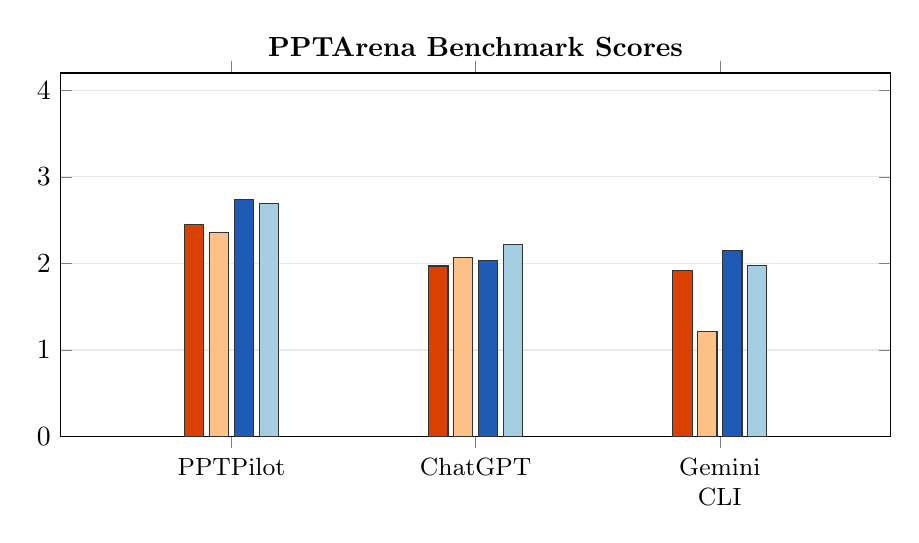
\begin{tikzpicture}
            \begin{axis}[
                ybar,
                width=\linewidth,
                height=6.2cm,
                bar width=7pt,
                ymin=0, ymax=4.2,
                ymajorgrids,
                grid style={gray!18},
                % INCREASED SPACING HERE
                enlarge x limits=0.35,
                symbolic x coords={PPTPilot,ChatGPT,GeminiCLI},
                xtick=data,
                xticklabels={PPTPilot,ChatGPT,Gemini\\CLI},
                xticklabel style={font=\small, text width=2.4cm, align=center},
                title={\textbf{PPTArena Benchmark Scores}},
                title style={yshift=-0.8ex},
            ]
                % ADDED DRAW=BLACK!80 FOR OUTLINES
                % 1. Gemini IF
                \addplot[fill=GeminiIF, draw=black!80] coordinates {
                    (PPTPilot,2.45) (ChatGPT,1.97) (GeminiCLI,1.92)
                };
                % 2. GPT-5 IF
                \addplot[fill=GPTIF, draw=black!80] coordinates {
                    (PPTPilot,2.36) (ChatGPT,2.07) (GeminiCLI,1.21)
                };
                % 3. Gemini VQ
                \addplot[fill=GeminiVQ, draw=black!80] coordinates {
                    (PPTPilot,2.74) (ChatGPT,2.03) (GeminiCLI,2.15)
                };
                % 4. GPT-5 VQ
                \addplot[fill=GPTVQ, draw=black!80] coordinates {
                    (PPTPilot,2.69) (ChatGPT,2.22) (GeminiCLI,1.98)
                };
            \end{axis}
        \end{tikzpicture}
    \end{minipage}%
    \hfill
    % --- 3. RIGHT PLOT ---
    \begin{minipage}[t]{0.45\textwidth}
        \centering
        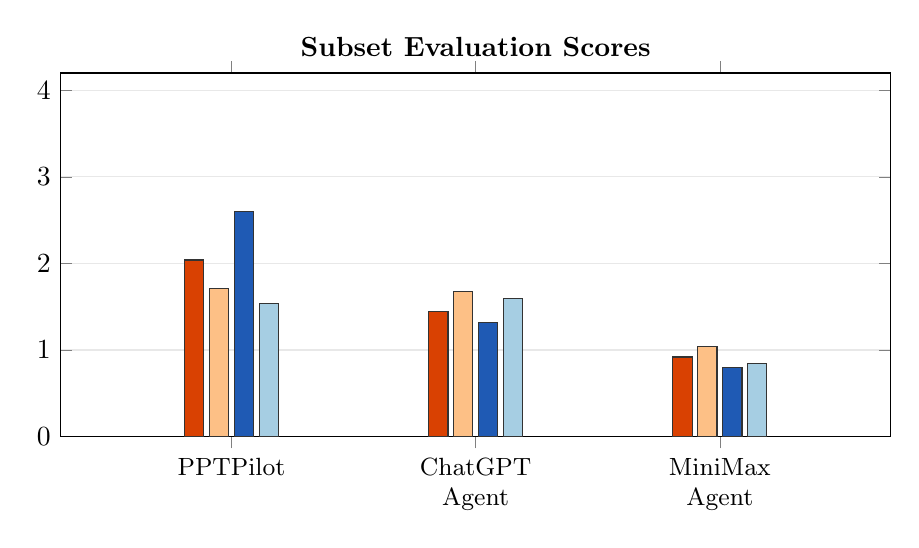
\begin{tikzpicture}
            \begin{axis}[
                ybar,
                width=\linewidth,
                height=6.2cm,
                bar width=7pt,
                ymin=0, ymax=4.2,
                ymajorgrids,
                grid style={gray!18},
                % INCREASED SPACING HERE
                enlarge x limits=0.35,
                symbolic x coords={PPTPilot,ChatGPTAgent,MiniMaxAgent},
                xtick=data,
                xticklabels={PPTPilot,ChatGPT\\Agent,MiniMax\\Agent},
                xticklabel style={font=\small, text width=2.6cm, align=center},
                title={\textbf{Subset Evaluation Scores}},
                title style={yshift=-0.8ex},
                legend columns=4, 
                legend to name=CommonLegend, 
                legend style={
                    draw=none, 
                    fill=none, 
                    font=\footnotesize,
                    /tikz/every even column/.append style={column sep=0.5cm}
                }
            ]
                % ADDED DRAW=BLACK!80 FOR OUTLINES
                % 1. Gemini IF
                \addplot[fill=GeminiIF, draw=black!80] coordinates {(PPTPilot,2.04) (ChatGPTAgent,1.44) (MiniMaxAgent,0.92)};
                \addlegendentry{Gemini IF (Dark Orange)}

                % 2. GPT-5 IF
                \addplot[fill=GPTIF, draw=black!80] coordinates {(PPTPilot,1.71) (ChatGPTAgent,1.68) (MiniMaxAgent,1.04)};
                \addlegendentry{GPT-5 IF (Light Orange)}

                % 3. Gemini VQ
                \addplot[fill=GeminiVQ, draw=black!80] coordinates {(PPTPilot,2.60) (ChatGPTAgent,1.32) (MiniMaxAgent,0.80)};
                \addlegendentry{Gemini VQ (Dark Blue)}

                % 4. GPT-5 VQ
                \addplot[fill=GPTVQ, draw=black!80] coordinates {(PPTPilot,1.54) (ChatGPTAgent,1.60) (MiniMaxAgent,0.84)};
                \addlegendentry{GPT-5 VQ (Light Blue)}
            \end{axis}
        \end{tikzpicture}
    \end{minipage}

    \caption{\textbf{Average IF/VQ scores visualized by judge.} We compare Instruction Following (Orange) and Visual Quality (Blue) across agents. Darker bars represent the Gemini Judge; lighter bars represent the GPT-5 Judge. The legend at the top applies to both charts.}
    \label{fig:gemini_barplots}
\end{figure*}


\begin{figure*}[!t]
    \centering
    \small
    
    % --- LEFT BLOCK (Contains 4 cases in a 2x2 grid) ---
    \begin{minipage}[t]{0.66\linewidth}
        % --- Row 1 of Left Block ---
        % Case 1: Layout & Captions
        \begin{minipage}[t]{0.48\linewidth}
            \centering
            \textbf{Create Layout and Add Captions}
            \vspace{0.2em}
            \includegraphics[width=\linewidth]{figures/Case12Original.png}\\[-0.25em]
            \textit{\scriptsize Original}\\[0.4em]
            \vspace{0.4em}
            \includegraphics[width=\linewidth]{figures/Case12GT.png}\\[-0.1em]
            \textit{\scriptsize Ground Truth}
        \end{minipage}
        \hfill
        % Case 2: Image Size
        \begin{minipage}[t]{0.48\linewidth}
            \centering
            \textbf{Correct Image Size \& Caption}
            \vspace{0.2em}
            \includegraphics[width=\linewidth]{figures/Case16Original.png}\\[-0.25em]
            \textit{\scriptsize Original}\\[0.4em]
            \vspace{0.4em}
            \includegraphics[width=\linewidth]{figures/Case16GT.png}\\[-0.1em]
            \textit{\scriptsize Ground Truth}
        \end{minipage}
        
        \vspace{1.5em} % Vertical gap between rows
        
        % --- Row 2 of Left Block ---
        % Case 3: Financials
        \begin{minipage}[t]{0.48\linewidth}
            \centering
            \textbf{Fix Chart Theme \& Formatting}
            \vspace{0.2em}
            \includegraphics[width=\linewidth]{figures/PPTPilotOriginal.png}\\[-0.25em]
            \textit{\scriptsize Original}\\[0.4em]
            \vspace{0.4em}
            \includegraphics[width=\linewidth]{figures/PPTPilotPrediction.png}\\[-0.1em]
            \textit{\scriptsize Ground Truth}
        \end{minipage}
        \hfill
        % Case 4: Research Poster
        \begin{minipage}[t]{0.48\linewidth}
            \centering
            \textbf{Organize Research Poster}
            \vspace{0.2em}
            \includegraphics[width=0.85\linewidth]{figures/OrganizeResearchPoster_TestA.pdf}\\[-0.25em]
            \textit{\scriptsize Original}\\[0.4em]
            \vspace{0.4em}
            \includegraphics[width=0.85\linewidth]{figures/OrganizeResearchPoster_GroundTruthA.pdf}\\[-0.1em]
            \textit{\scriptsize Ground Truth}
        \end{minipage}
    \end{minipage}
    \hfill
    % --- RIGHT BLOCK (Single tall column for Complex Collage) ---
    \begin{minipage}[t]{0.32\linewidth}
        \centering
        \textbf{Complex Collage Layout}
        \vspace{0.2em}
        
        % Group 1: The two Original Images
        \includegraphics[width=\linewidth]{figures/Case17Test1.png}\\[0.2em]
        \includegraphics[width=\linewidth]{figures/Case17Test2.png}\\[-0.1em]
        \textit{\scriptsize Original Assets}
        
        \vspace{0.8em} % Gap between inputs and outputs
        
        % Group 2: The two Ground Truth Images
        \includegraphics[width=\linewidth]{figures/Case17GT1.png}\\[0.2em]
        \includegraphics[width=\linewidth]{figures/Case17GT2.png}\\[-0.1em]
        \textit{\scriptsize Ground Truth}
    \end{minipage}

    \vspace{0.5em}
    \caption{Cases from our PPTArena Benchmark showing significant visual complexity. The left columns illustrate specific tasks (layout, sizing, charts, posters), while the right column demonstrates a complex multi-slide collage task where multiple assets are harmonized into a cohesive theme.}
    \label{fig:moreimages_cases}
\end{figure*}




\onecolumn

\section*{Appendix II Code Listings}
\addcontentsline{toc}{section}{Appendix II Code Listings}

\nolinenumbers

\noindent
\begin{lstlisting}[caption={PPTX to JSON Conversion Logic}, label={lst:pptx_to_json}, language=Python]
def pptx_to_json(filepath):
    """
    Converts a .pptx file to a comprehensive JSON representation.
    Captures all edit types: Content, Layout, Styling, Interactivity, and Structure.
    """
    try:
        prs = Presentation(filepath)
        
        # Presentation-level metadata
        presentation_data = {
            "filename": os.path.basename(filepath),
            "slide_width": prs.slide_width.pt if hasattr(prs, 'slide_width') else None,
            "slide_height": prs.slide_height.pt if hasattr(prs, 'slide_height') else None,
            "slides": []
        }
        
        # ... [Metadata extraction logic omitted for brevity] ...
        
        for i, slide in enumerate(prs.slides):
            slide_data = {
                "slide_number": i + 1,
                "shapes": [],
                "notes": "",
                # Layout & Structure info
                "slide_layout": slide.slide_layout.name if hasattr(slide, 'slide_layout') else None,
                "slide_id": slide.slide_id if hasattr(slide, 'slide_id') else None,
            }
            
            # ... [Shape iteration and property extraction logic omitted for brevity] ...
            # ... [Captures: Background, Shapes, Text, Tables, Images, Charts, Groups] ...
            
            presentation_data["slides"].append(slide_data)
            
        return presentation_data
    except Exception as e:
        print(f"Error processing {filepath}: {e}")
        return None
\end{lstlisting}
\vspace{1cm}


\noindent
\begin{lstlisting}[caption={Smart Diff Construction}, label={lst:smart_diff}, language=Python]
def diff_pptx_json(ground_truth_json, prediction_json, initial_json=None):
    """
    Performs a deep comparison between ground_truth and prediction JSON structures.
    Returns a structured diff with only the differences, organized by slide and shape.
    """
    differences = []
    
    # ... [Helper functions: normalize_value, values_match, compare_dict, compare_list omitted] ...
    
    # Compare slides
    gt_slides = ground_truth_json.get("slides", [])
    pred_slides = prediction_json.get("slides", [])
    init_slides = initial_json.get("slides", []) if initial_json else []
    
    for slide_idx in range(max(len(gt_slides), len(pred_slides))):
        # ... [Slide comparison logic omitted] ...
        pass
    
    # Calculate similarity score
    total_properties = len(differences) + 100  # Baseline to avoid division by zero
    similarity_score = 1.0 - (len(differences) / total_properties)
    
    return {
        "has_differences": len(differences) > 0,
        "similarity_score": max(0.0, min(1.0, similarity_score)),
        "total_differences": len(differences),
        "differences": differences
    }
\end{lstlisting}

\clearpage

\noindent
\begin{lstlisting}[caption={Style Target Generation Prompt}, label={lst:style_prompt}]
You are an expert technical writer for presentation editing workflows.
Given ONLY the Original deck and the Ground Truth deck, produce actionable, specific instructions to convert Original into Ground Truth. Focus on content and structure inferred from JSON; do not reference any predictions.

--- ORIGINAL (JSON summary) ---
```json
{original_ppt_json_truncated}
```

--- GROUND TRUTH (JSON summary) ---
```json
{ground_truth_ppt_json_truncated}
```

Return a single JSON object with keys: overview_instructions (multi-sentence, stepwise where helpful), and notes (optional).
\end{lstlisting}
\vspace{1cm}

\nolinenumbers
\noindent
\begin{lstlisting}[caption={Full Instruction Following Judge Prompt}, label={lst:if_prompt}]
You are a strict judge of INSTRUCTION FOLLOWING.

CRITICAL UNDERSTANDING:
- The "Instruction" is what the model/editor received (the user's request)
- The "Style Target" is YOUR evaluation rubric - the model DID NOT see this
- You will receive a FOCUSED DIFF showing only what changed between ground_truth and prediction
- Your job: Judge if the prediction's changes match the ground_truth's changes
- DO NOT compare prediction to initial - focus on whether prediction achieved ground_truth's outcome
- If the diff shows minimal differences, that's GOOD (high score)
- Ground Truth is ONE valid example, not the only correct answer

FLEXIBILITY:
- Accept different valid approaches (e.g., flags in a list vs rows is fine if they match the text)
- Exact positions/sizes don't matter unless the Instruction explicitly requires them
- Very small measurement variations ($\pm$1%) are acceptable for fonts/sizes due to rounding
- Z-order (layering) differences ARE significant and should be noted
- Focus on semantic properties: text content, font names, colors, structural changes, z-order

HARSH SCORING POLICY (very strict):
- Choose the lower score when uncertain between adjacent scores.
- For translation/summarization or other text edits requiring reasoning, semantic similarity is more important than exact wording.

INSTRUCTION_FOLLOWING score (0-5):
- 5: Every requested object/change exists and is exactly correct; nothing requested is missing or misapplied; no extra edits beyond the instruction.
- 4: All requested changes exist and are mostly correct; only a tiny inaccuracy that does not affect meaning.
- 3: Most requested changes exist but at least one is incomplete, incorrect, or missing detail.
- 2: Only some requested changes exist; notable misses or incorrect applications.
- 1: Requested changes largely not performed or substantially incorrect.
- 0: Contradicts or ignores the instruction entirely.

Output a single JSON object with:
- instruction_following_score (0-5)
- instruction_following_reason (one sentence, specific evidence comparing prediction to ground_truth)

--- USER INSTRUCTION (what the model received) ---
{instruction_part}

--- STYLE TARGET (your evaluation rubric - the model DID NOT see this) ---
{style_target_part}

--- SMART DIFF ANALYSIS (Prediction vs Ground Truth) ---
{formatted_diff}

CRITICAL COMPARISON INSTRUCTIONS:
The diff above shows ONLY the differences between prediction and ground_truth.
- If the diff shows "No differences" $\rightarrow$ Perfect match $\rightarrow$ Score 5
- If the diff shows differences in properties that the instruction requires $\rightarrow$ Score based on correctness
- Focus on whether prediction achieved the same semantic outcome as ground_truth

REMINDER: Judge if the prediction achieved the SEMANTIC INTENT of the Instruction.
The diff highlights what actually changed - use this to make an accurate judgment.
\end{lstlisting}

\clearpage

\nolinenumbers
\noindent
\begin{lstlisting}[caption={Full Visual Quality Judge Prompt}, label={lst:vq_prompt}]
You are a judge of VISUAL/CONTENT QUALITY and PRESERVATION.

CRITICAL UNDERSTANDING:
- The "Instruction" is what the model/editor received
- The "Style Target" is YOUR evaluation rubric - the model DID NOT see this
- Ground Truth is ONE valid example - accept other valid visual approaches
- Focus on SEMANTIC correctness: Are the visual elements correct? No overlap? Readable?
- Exact positions/sizes don't matter unless the Instruction explicitly requires them
- You will only receive Ground Truth and Prediction slide images; compare them directly slide-by-slide.
- Use any provided Style Target guidance to check required visual cues strictly.

FLEXIBILITY:
- Different layouts achieving the same goal are acceptable (e.g., list vs grid)
- Small position variations are fine if elements are clear and non-overlapping
- Theme colors may vary slightly as long as they're harmonious
- "Approximately centered" or "well-aligned" is acceptable without pixel-perfection

HARSH SCORING POLICY (very strict):
- Penalize any unintended visual change to non-requested content (fonts, sizes, colors, positions, shapes, charts, images, tables, or slide structure).
- Choose the lower score when uncertain between adjacent scores.

VISUAL_Quality score (0-5):
- 5: No unintended changes to non-requested content; fonts, sizes, colors, positions, and objects match Ground Truth; structure preserved.
- 4: Visually very close to the Ground Truth; only imperceptible or negligible differences (e.g., sub-pixel alignment); no style drift.
- 3: Minor but noticeable visual differences (e.g., slight font weight/size/spacing shifts) without breaking layout.
- 2: Clear deviations (e.g., wrong fonts/sizes/colors, noticeable position shifts) or small layout issues.
- 1: Major deviations (overlap, off-canvas, broken layout) but still legible.
- 0: Severely broken or unreadable slide.

Output a single JSON object with:
- visual_quality_score (0-5)
- visual_quality_reason (one sentence, specific evidence about visual differences)

--- User Instruction ---
{instruction_text}

--- Style Target (judge rubric, unseen by the model under evaluation) ---
{style_block}

You are given two labeled image sequences:
- Ground Truth: the correct target deck to match
- Prediction: the candidate deck produced by the system

CRITICAL: Ground Truth is ONE valid example, not the only correct answer.
Judge if Prediction achieves the SEMANTIC INTENT shown by Ground Truth.
Accept different valid layouts/arrangements that fulfill the instruction and style target.
Focus on: correctness, no overlap, readability, theme consistency.
Small position/size variations are acceptable if elements are clear.

Judge visual quality by comparing PREDICTION to GROUND TRUTH.

Return only:
- visual_quality_score (0-5)
- visual_quality_reason (one sentence, specific evidence about visual differences)
\end{lstlisting}
\linenumbers